%\subsubsection*{Plasma Fusion simulations}

%The largest community that uses ADIOS is of the plasma fusion simulations, as several fusion scientists have been collaborating with the ADIOS team and used the library in their applications from the beginning, giving invaluable insight for the ADIOS team in the works of many large scale simulations. Particle simulation based fusion applications that can utilize the largest  supercomputers (i.e. several hundreds of thousands of cores today), like XGC1, GTC and GTC-P all use ADIOS for writing the large checkpoint/restart data as well as the small but frequent diagnostic data. ADIOS played center role in coupling multiple fusion codes together for creating a multi-scale multi-physics fusion simulation~\cite{ADIOS:Docan:ccgrid10}. The separate codes used ADIOS to write and read data that was transferred between the codes directly without writing files. Magneto-hydrodynamic codes like M3D-K, M3D-C1 and GEM also use ADIOS for checkpoint/restart because they had I/O bottlenecks already at a few hundred cores. The output of M3D was also changed to ADIOS in order to feed that data into XGC in a fusion coupling scenario. 


ADIOS/DataSpaces~\cite{ADIOS:Docan:cluster12} is a scalable data-staging substrate that supports advanced coordination and interaction services for extreme scale coupled simulation workflows. It provides the abstractions and mechanisms to support flexible and dynamic inter-application coupling and interactions at runtime, and supports asynchronous data insertion and retrieval to/from a staging area composed of a set of cores on application nodes and dedicated staging nodes. For example, in case of a simulation-visualization workflow, the simulation can output data to the staging resources at runtime using the DataSpaces put() operator, and the visualization processes can asynchronously fetch relevant portions of the data using the corresponding get() operator. Note that these operators are independent of the scale and the distribution of these interacting applications. The internal data management mechanisms in DataSpaces ensure the scalability of the distributed data storage and lookup mechanisms. The DataSpaces runtime builds on DART~\cite{ADIOS:Docan:ccpe10} enables direct low-overhead, high-throughput memory-to-memory communication between the interacting nodes using Remote Direct Memory Access (RDMA). 

DataSpaces implements a distributed query engine with simple and flexible query semantics to facilitate access to the data. An application component can query any data region from the global application domain, e.g., an individual, or a range of data points. Extending the query engine, DataSpaces builds higher-level data sharing and coupling abstractions to support complex and dynamic interaction and coupling patterns. Applications can query data regions on-demand, register to obtain continuous notifications of data availability, implement the publisher-subscriber programming paradigm, share and redistribute data in a decoupled manner, and move analytics code to the data.

DataSpaces consists of two main components: a client module used by the ADIOS/DataSpaces method, and a DataSpaces server module. The client library is light-weight and provides an asynchronous I/O API. It is integrated with ADIOS and the functionality is exposed through the ADIOS write/read semantics, which bundles the variables of the same output together, so that reading applications can access a set of variables of an output step consistently just like when reading from files.

ADIOS/DataSpaces is currently used in production in coupled scientific simulation workflows on large-scale supercomputers. For example, as part of the fusion simulation framework (Figure~\ref{part3-ch5-adios:fig:coupling}), DataSpaces enables memory-to-memory coupling between the gyrokinetic PIC edge simulation code XGC0, and the MHD code M3D-OMP~\cite{ADIOS:Docan:ccgrid10}. Similarly, as part of the turbulent combustion workflow DataSpaces enables data coupling between the direct numerical simulations (DNS) code S3D and the data analytics pipeline~\cite{ADIOS:Bennett:SC12}.

\begin{figure}[h!]
\centering
\myIfColor
{
% use color version
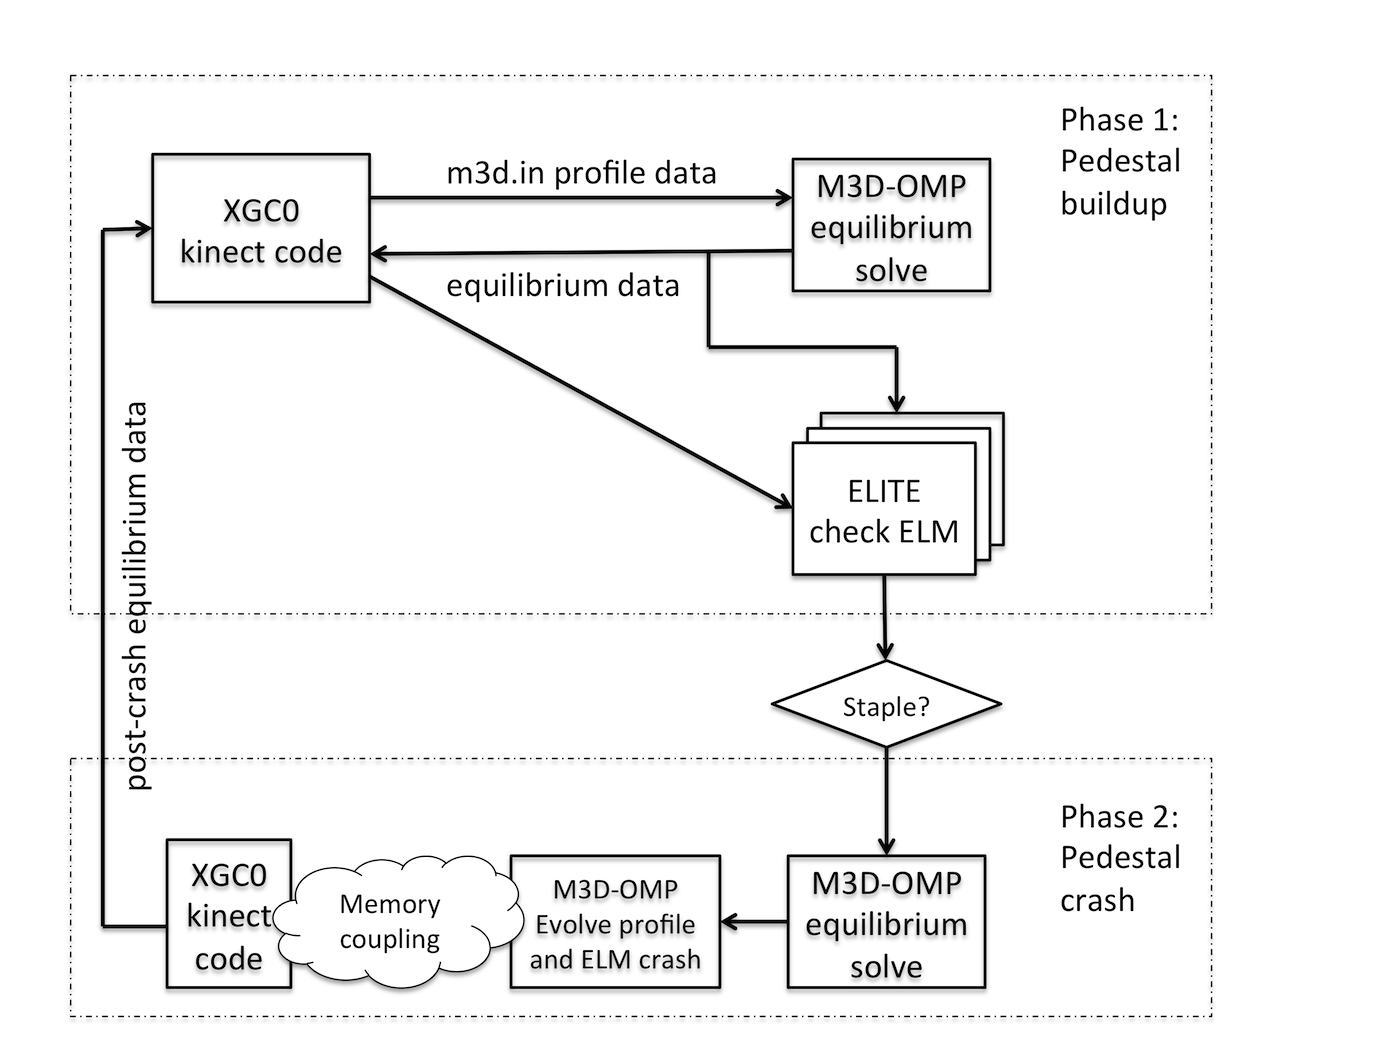
\includegraphics[width=0.7\textwidth]{Chapters/part3-ch5-adios/figs/coupling.png}
}
{
% use B&W version
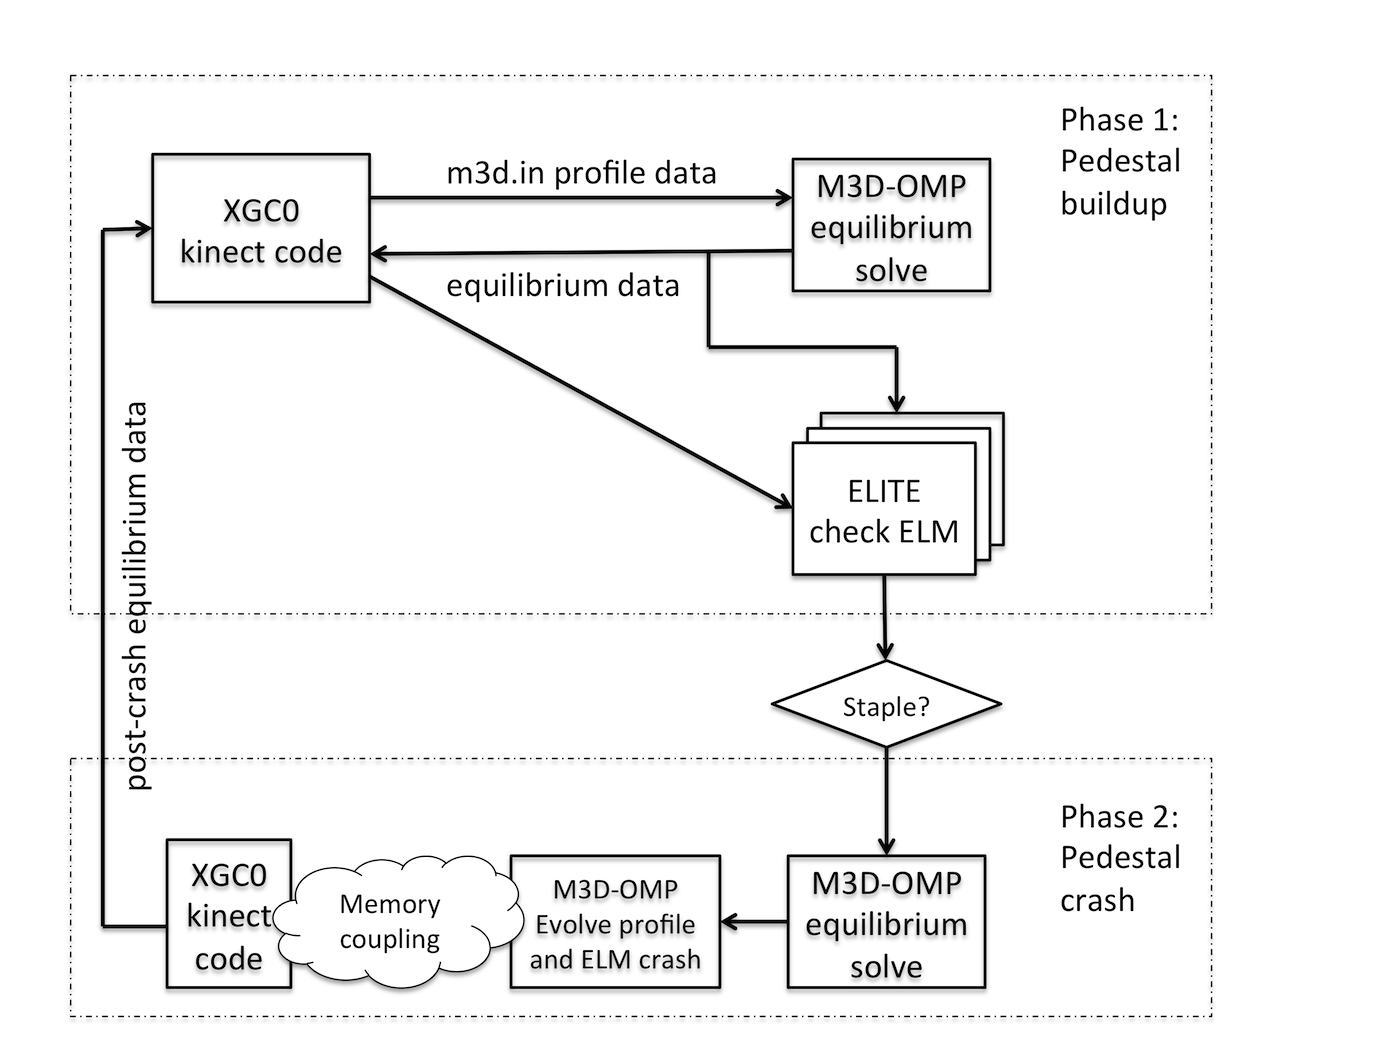
\includegraphics[width=0.7\textwidth]{Chapters/part3-ch5-adios/figs/coupling.png}
}
\caption[]
{Coupled Fusion Simulation Workflow using ADIOS and DataSpaces.
}
\label{part3-ch5-adios:fig:coupling}
\end{figure}